\documentclass[10pt, aspectratio=1610]{beamer}

% Packages requis
\usepackage[utf8]{inputenc}
\usepackage[T1]{fontenc}
\usepackage{lmodern}
\usepackage{babel}
\babelprovide[import,main]{french}
\usepackage{graphicx}
\usepackage{booktabs}
\usepackage{amsmath}
\usepackage{tikz}
\usetikzlibrary{shapes, arrows.meta, positioning, calc, chains, shadows, fit}
\usepackage{caption}

% --- Configuration du Thème (Style Université de Bordeaux) ---
\usetheme{Madrid}
\usecolortheme{dolphin}

% Définition des couleurs approximatives de l'Université de Bordeaux
\definecolor{UnivBlue}{RGB}{0, 51, 102}   % Bleu fonce
\definecolor{UnivRed}{RGB}{153, 0, 0}     % Rouge/Bordeaux
\definecolor{LayerBlue}{RGB}{200, 220, 255}
\definecolor{LayerRed}{RGB}{255, 200, 200}
\definecolor{LayerGreen}{RGB}{200, 255, 200}
\definecolor{LayerYellow}{RGB}{255, 255, 200}

% Application des couleurs
\setbeamercolor{structure}{fg=UnivBlue}
\setbeamercolor{palette primary}{bg=UnivBlue, fg=white}
\setbeamercolor{palette secondary}{bg=UnivBlue!80, fg=white}
\setbeamercolor{palette tertiary}{bg=UnivBlue!60, fg=white}
\setbeamercolor{frametitle}{bg=UnivBlue, fg=white}
\setbeamercolor{title}{bg=UnivBlue, fg=white}
\setbeamercolor{block title}{bg=UnivBlue, fg=white}
\setbeamercolor{alerted text}{fg=UnivRed}

% --- Styles TikZ pour les architectures ---
\tikzset{
    block/.style={rectangle, draw, fill=white, align=center, rounded corners, drop shadow, font=\scriptsize},
    conv/.style={block, fill=LayerBlue, minimum height=2em},
    pool/.style={block, fill=LayerRed, minimum height=1.5em},
    dense/.style={block, fill=LayerGreen, minimum height=2em},
    op/.style={circle, draw, fill=LayerYellow, inner sep=1pt, font=\tiny},
    arrow/.style={-{Stealth[scale=1.0]}, thick, color=UnivBlue},
    label/.style={font=\tiny, color=gray}
}

% --- Informations de la présentation ---
\title[multi-expert-peptide-pipeline]{ Multi Expert Peptide Pipeline}
\subtitle{Projet de fin d'études}
\author[N.F \& E.I \& A.M \& N.R]{Nathan Fitger \and Eduard Iliescu \and Arthur Macdonald \and Niels Roudeau \\[1em]
{\small Supervisé par : Johan Samot (UB), Enzo Edderbah (ISM) et Akka Zemmari (UB/LABRI)}}
\institute[Université de Bordeaux]{
    Université de Bordeaux \\
    Master 2 Informatique — Intelligence Artificielle
}
\date{Année 2025—2026}

% Define custom minimize command
\newcommand{\minimize}[1]{\textit{\footnotesize #1}}

% --- Person marker dots (slide ownership) ---
% Usage inside a frame:
%   \persondotleft{NathanColor}
%   \persondotright{EduardColor}
\definecolor{NathanColor}{RGB}{55, 170, 55}
\definecolor{EduardColor}{RGB}{180, 55, 180}
\definecolor{ArthurColor}{RGB}{170, 170, 55}
\definecolor{NielsColor}{RGB}{180, 55, 55}

\newcommand{\persondotleft}[2][2.8pt]{%
    \begin{tikzpicture}[remember picture,overlay]
        \fill[#2] ([xshift=0.55cm,yshift=-0.55cm]current page.north west) circle (#1);
    \end{tikzpicture}%
}

\newcommand{\persondotright}[2][2.8pt]{%
    \begin{tikzpicture}[remember picture,overlay]
        \fill[#2] ([xshift=-0.55cm,yshift=-0.55cm]current page.north east) circle (#1);
    \end{tikzpicture}%
}

% Logo Placeholder
\titlegraphic{
    
\includegraphics[width=2cm]{images/ism.png}
    
\includegraphics[width=2cm]{images/ubordeaux.png}
    
\includegraphics[width=2cm]{images/LABRI_BIG_0.png}
}

\begin{document}

% 1. Slide de Titre
\begin{frame}
    \titlepage
\end{frame}

% Sommaire
\begin{frame}{Plan de la présentation}
    \persondotright[4pt]{NathanColor}
    \tableofcontents
\end{frame}

% --- Section 1: Présentation ---
\section{Contexte et objectifs}
\begin{frame}{Contexte et Objectifs}
    \begin{center}
        Pipeline agentique multi expert pour la découverte de peptides \textit{in silico}
        \\
        \footnotesize{in silico: réalisé par ordinateur, sans expérimentation physique.}
        \\
        \centering
        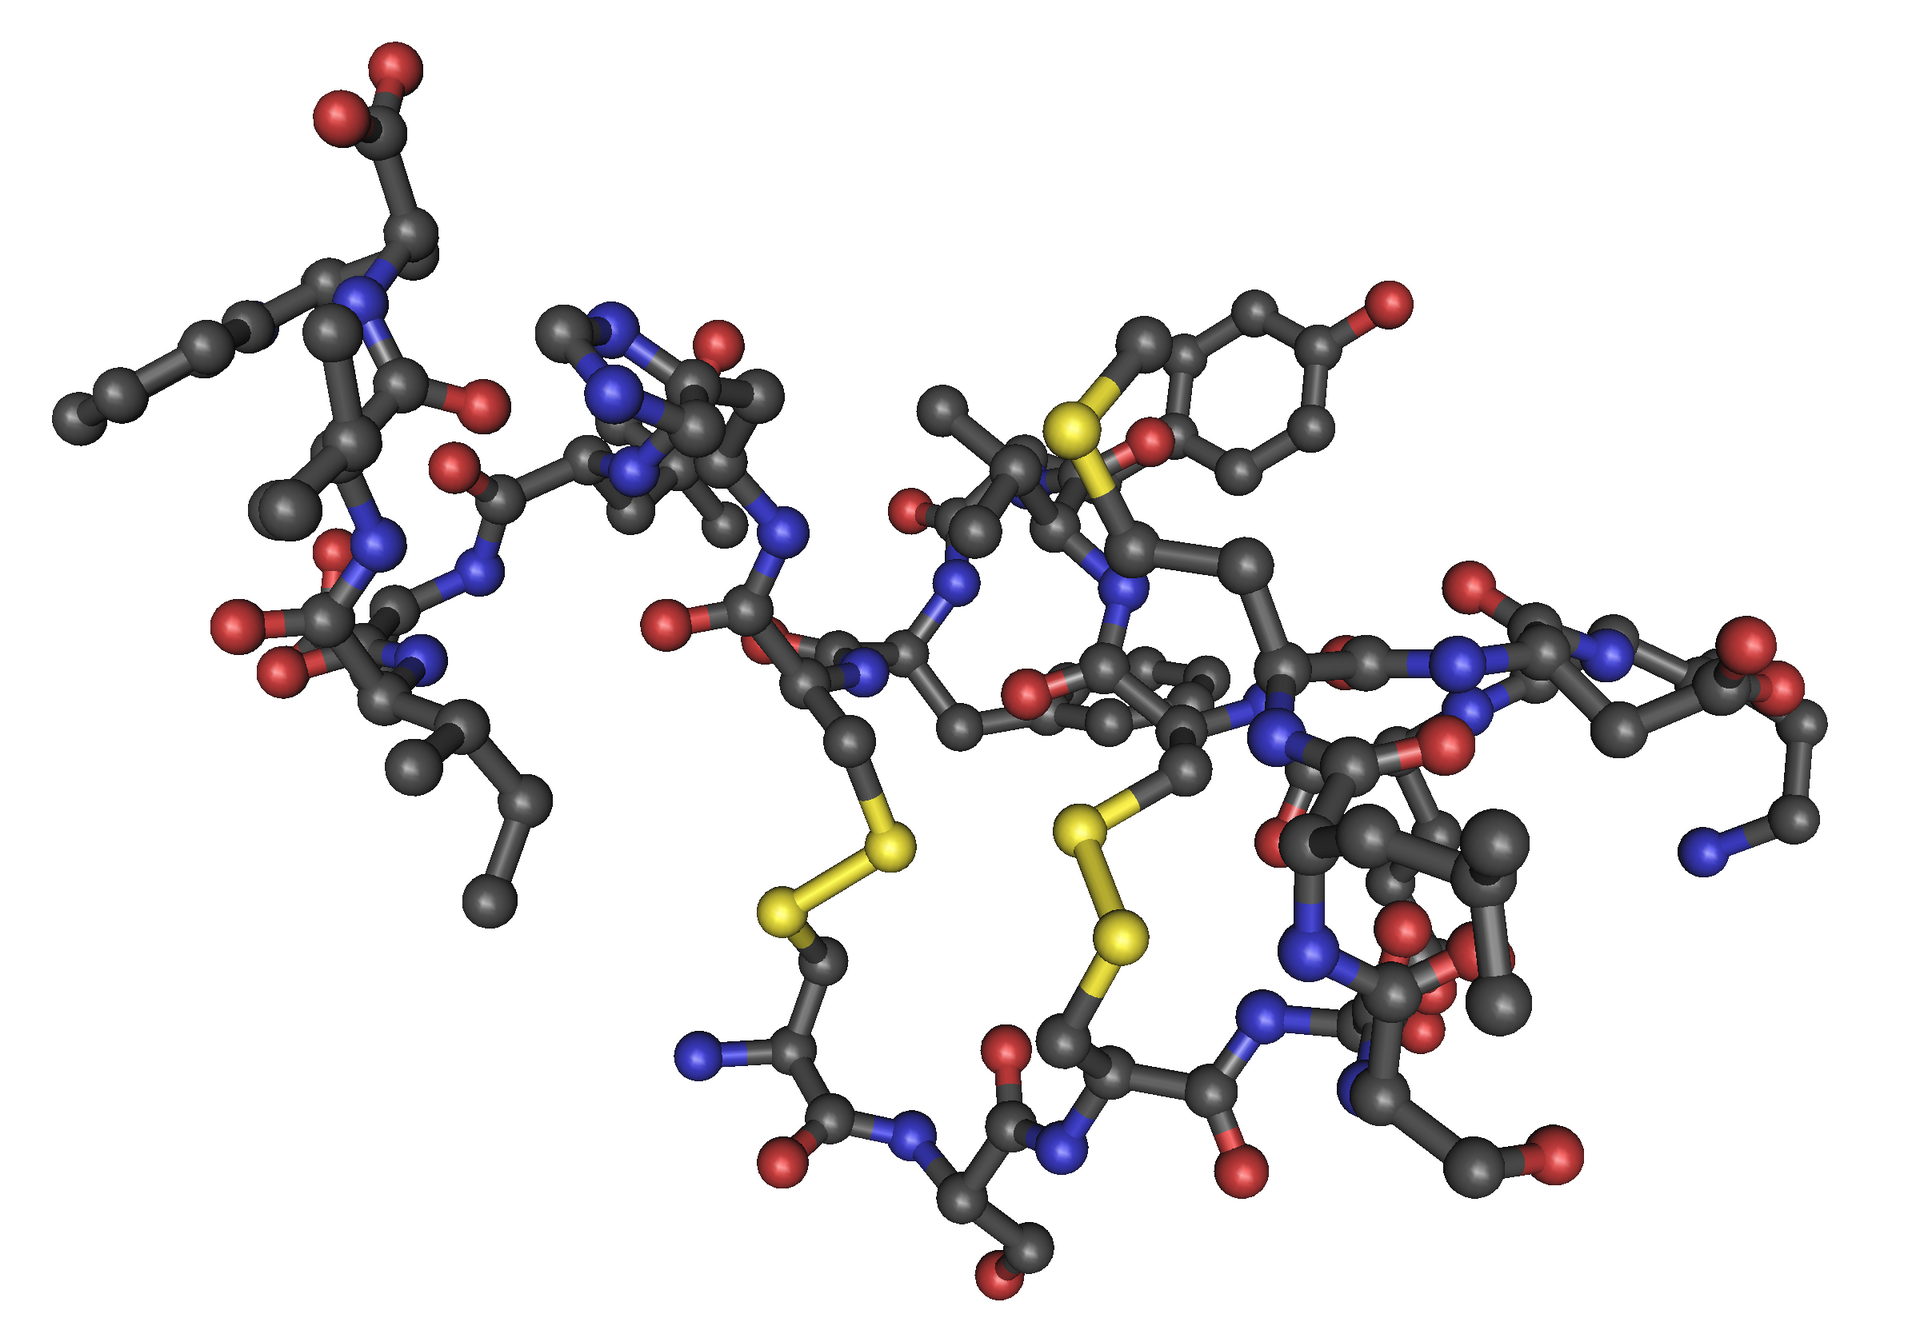
\includegraphics[height=4cm]{peptide.png}
    \end{center}
\end{frame}

\begin{frame}
    \frametitle{Peptide}
    \begin{itemize}
        \item Chaîne composée d'au plus 50 acides aminés
        \item 20 acides aminés différents
        \item Applications: médecine, agriculture, industrie
        \item Exemples: insuline, antibiotiques, hormones
    \end{itemize}

    \begin{block}{Processus de découverte actuel}
        \begin{itemize}
            \item Découverte de peptides: criblage de bibliothèques, évolution dirigée
            \item Évaluation: tests biologiques, simulations moléculaires
            \item Itération sur les resultats pour améliorer l'efficacité de la peptides
            \item Coût élevé, temps long, taux de succès faible
        \end{itemize}
    \end{block}
\end{frame}

\section{Experts et Architecture}
\begin{frame}
    \frametitle{Pipeline}
        \begin{center}
            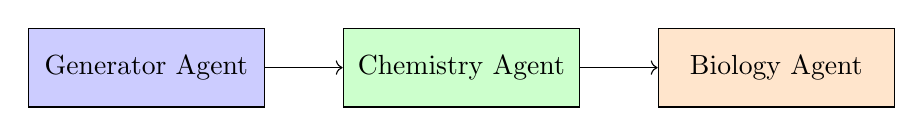
\begin{tikzpicture}
            \node[rectangle, draw, fill=blue!20, minimum width=3cm, minimum height=1cm, align=center] (gen) at (0, 0) {Generator Agent};
            \node[rectangle, draw, fill=green!20, minimum width=3cm, minimum height=1cm, align=center] (chem) at (4, 0) {Chemistry Agent};
            \node[rectangle, draw, fill=orange!20, minimum width=3cm, minimum height=1cm, align=center] (bio) at (8, 0) {Biology Agent};

            \draw[->] (gen) -- (chem);
            \draw[->] (chem) -- (bio); 
            \end{tikzpicture}
        \end{center}
\end{frame}
\subsection{Expert Générateur de peptides}
\begin{frame}
    \frametitle{Générateur}
    \begin{block}{Modèle du générateur}
        \begin{itemize}
        \item Modèle générant des séquences de peptides à partir de séquence ou propriétés souhaitées
        \item Entraîné sur une base de données de peptides connus et leurs propriétés
        \item Capable de générer des peptides avec des propriétés spécifiques (ex: propriétés chimiques)
        \end{itemize}
    \end{block}

    \begin{block}{Modèles implémentés}
        \begin{itemize}
        \item VAE (Variational Autoencoder): apprend une représentation latente des peptides et génère de nouvelles séquences à partir de cette représentation
        \item CVAE (Conditional Variational Autoencoder): extension du VAE qui conditionne la génération sur des propriétés spécifiques (propritétés physico-chimiques, activité biologique)
    \end{itemize}
    \end{block}
\end{frame}

\begin{frame}
    \frametitle{Résultats du générateur}
    \begin{block}{VAE et CVAE}
        \begin{itemize}
        \item Génération de peptides aléatoires à l'aide du VAE
        \end{itemize}
        \centering
        01: IWIGRK

        \begin{itemize}
        \item Génération de peptides à partir de trois propriétés différentes (longueur, cathionicity, hydrophobicity) à l'aide du CVAE
        \end{itemize}

        \centering
        01: KRACLIRRLR

        \begin{center}
        \begin{tabular}{|c|c|}
        \hline
        Lettre & Composition chimique \\
        \hline
        K & Lysine (K) \\
        R & Arginine (R) \\
        A & Alanine (A) \\
        C & Cysteine (C) \\
        L & Leucine (L) \\
        I & Isoleucine (I) \\
        \hline
        \end{tabular}
        \end{center}
    \end{block}
\end{frame}
\begin{frame}
    \begin{block}{Évaluation du générateur}
        \begin{itemize}
        \item Évaluation de la qualité des peptides générés en comparant leurs propriétés à celles des peptides connus
        \end{itemize}
        \centering
        Lorsqu'on donne la sequence KLFKRWKHLFR de taille 11 et ses propriétés physico-chimiques au CVAE, il génère la sequence RKLKLFFRLLR avec des propriétés similaires.

        \begin{itemize}
        \item Utilisation de métriques telles que la diversité, la validité et la nouveauté des séquences générées
        \end{itemize}
    \end{block}
\end{frame}



\subsection{Expert Chimiste}
\begin{frame}
    \frametitle{Chimiste}
    \begin{block}{Modèle du chimiste}
        \begin{itemize}
        \item Prend en entrée une ou des séquences de peptides générés par le générateur
        \item Prend des intervales de propriétés chimiques souhaitées 
        \item Utilise des règles chimiques et physiques pour donner un score à la peptide à partir des intervalles et cibles séléctionnés
        \end{itemize}
    \end{block}
    \begin{block}{Propriétés chimiques évaluées}
            Taille de la séquence, Poids moléculaire, Charge nette, LogP (coefficient de partage octanol-eau), Hydrophobicité, Point isoélectrique\dots
    \end{block}
    \begin{block}{Résultats du chimiste}
        \begin{itemize}
        \item propriétées chimiques des peptides générés par le générateur
        \item score basé sur la distance entre les propriétés chimiques des peptides générés et les cibles de propriétés souhaitées
        \item si la peptide est hors des intervalles de propriétés souhaitées, le score est pénalisé
    \end{itemize}
    \end{block}
\end{frame}
\subsection{Expert Biologiste}
\begin{frame}
    \frametitle{Biologiste}
    \begin{block}{Modèle du biologiste}
        \begin{itemize}
        \item Modèle d'embedding ESM-2 $\rightarrow$ représente les peptides et leurs propriétés biologiques dans un espace latent
        \item Modèle \textbf{esm2\_t12\_35M\_UR50D} par Facebook AI Research, entraîné sur une grande base de données de séquences protéiques (35M de paramètres).
        \item Basé sur des données biologiques afin d'apprendre les relations entre la structure des peptides l'activitée biologique
        \end{itemize}
    \end{block}
    \begin{block}{Modèle utilisé}
        \begin{itemize}
            \item Affinité pour une cible spécifique (\textbf{Exemple: une souche bactérienne})
            \item Activité antimicrobienne
            \item Toxicité potentielle
            \item Stabilité dans des conditions biologiques
        \end{itemize}
    \end{block}
\end{frame}
\subsection{Architecture du pipeline multi-expert}
\begin{frame}
    \persondotright[4pt]{EduardColor}
    \frametitle{Architecture du pipeline multi-expert}
    \begin{figure}[h]
    \centering
    \resizebox{0.75\textwidth}{!}{%
    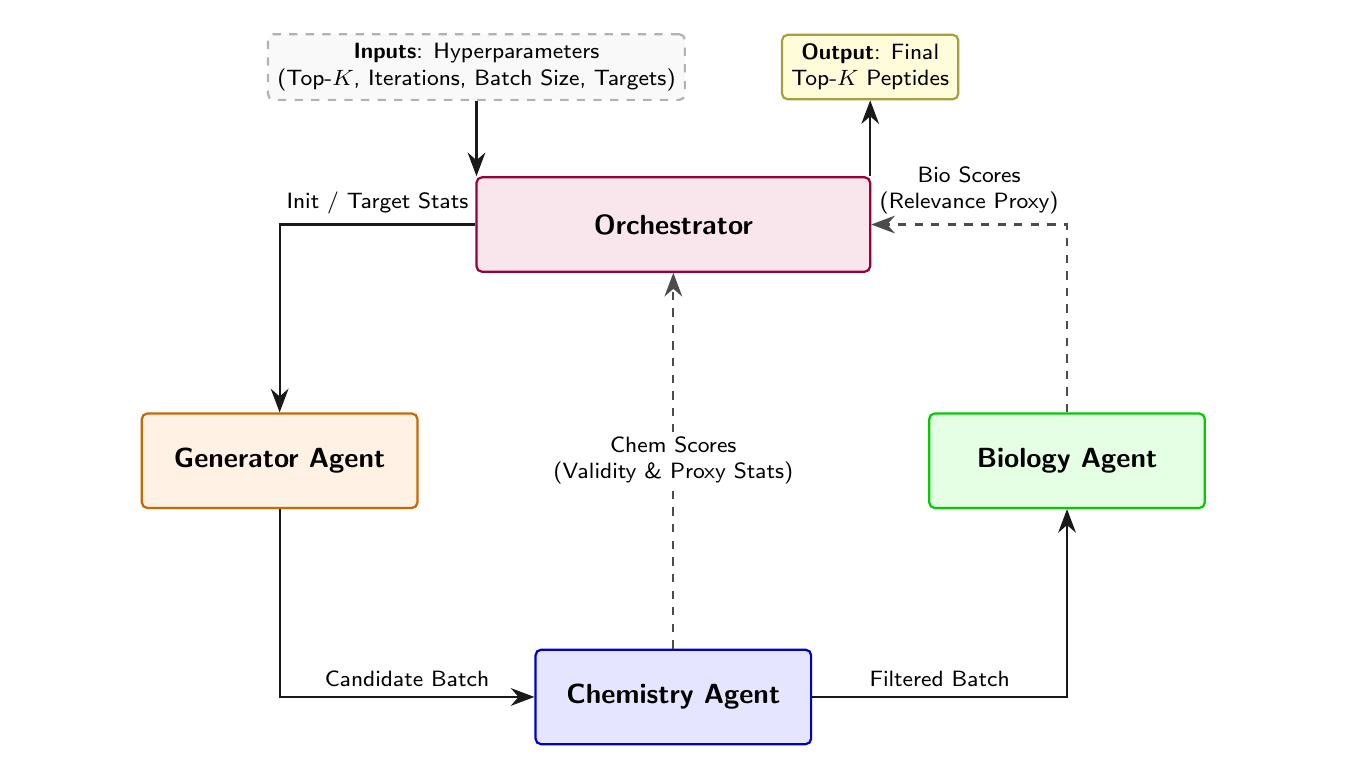
\begin{tikzpicture}[
        >=latex,
        % Base Agent Style
        agent/.style={
            rectangle,
            thick,
            minimum width=3.5cm,
            minimum height=1.2cm,
            align=center,
            font=\sffamily\bfseries,
            rounded corners=2pt
        },
        % Distinct Professional Colors for each Agent
        orchStyle/.style={agent, fill=purple!10, draw=purple!80!black, minimum width=5cm},
        genStyle/.style={agent, fill=orange!10, draw=orange!80!black},
        chemStyle/.style={agent, fill=blue!10, draw=blue!80!black},
        bioStyle/.style={agent, fill=green!10, draw=green!80!black},
        % Input / Output Styles
        io/.style={rectangle, thick, align=center, font=\sffamily\footnotesize, rounded corners=2pt},
        inputStyle/.style={io, dashed, fill=gray!5, draw=gray!60},
        outputStyle/.style={io, solid, fill=yellow!15, draw=yellow!60!black},
        % Flow Lines
        batchFlow/.style={-{Stealth[length=3mm]}, thick, draw=black!90},
        scoreFlow/.style={-{Stealth[length=3mm]}, thick, dashed, draw=black!70}
    ]

    % --- NODES ---
    \node[orchStyle] (orch) at (0, 3) {Orchestrator};
    \node[genStyle]  (gen)  at (-5, 0) {Generator Agent};
    \node[chemStyle] (chem) at (0, -3) {Chemistry Agent};
    \node[bioStyle]  (bio)  at (5, 0) {Biology Agent};

    % --- SYSTEM INPUTS & OUTPUTS ---
    \node[inputStyle] (inputs) at (-2.5, 5) {\textbf{Inputs}: Hyperparameters\\(Top-$K$, Iterations, Batch Size, Targets)};
    \node[outputStyle] (outputs) at (2.5, 5) {\textbf{Output}: Final\\Top-$K$ Peptides};

    % Connect IO to Orchestrator (Straight up/down)
    \draw[batchFlow] (inputs) -- (inputs |- orch.north);
    \draw[batchFlow] (outputs |- orch.north) -- (outputs);

    % --- BATCH DATA FLOW (Solid Lines) ---
    % 1. Orchestrator -> Generator
    \draw[batchFlow] (orch.west) -| node[pos=0.25, above, font=\sffamily\footnotesize, align=center] {Init / Target Stats} (gen.north);

    % 2. Generator -> Chemistry
    \draw[batchFlow] (gen.south) |- node[pos=0.75, above, font=\sffamily\footnotesize, align=center] {Candidate Batch} (chem.west);

    % 3. Chemistry -> Biology
    \draw[batchFlow] (chem.east) -| node[pos=0.25, above, font=\sffamily\footnotesize, align=center] {Filtered Batch} (bio.south);

    % --- FEEDBACK & SCORE FLOW (Dashed Lines) ---
    % 4. Chemistry -> Orchestrator (Straight up through the center)
    \draw[scoreFlow] (chem.north) -- node[fill=white, inner sep=2pt, font=\sffamily\footnotesize, align=center] {Chem Scores\\(Validity \& Proxy Stats)} (orch.south);

    % 5. Biology -> Orchestrator
    \draw[scoreFlow] (bio.north) |- node[pos=0.75, above, font=\sffamily\footnotesize, align=center] {Bio Scores\\(Relevance Proxy)} (orch.east);

    % Enforce a symmetric final bounding box around x=0 to guarantee true global centering.
    \pgfresetboundingbox
    \path (-8.2, -3.4) rectangle (8.2, 5.5);

    \end{tikzpicture}
    }
    \caption{Agentic Pipeline Architecture. }
    \end{figure}
\end{frame}
\input{sections/06_Interface.tex}
\section{Résultats et évaluation du pipeline}
\begin{frame}
    \frametitle{Résultats: effet des itérations et du batch}
    \begin{columns}[T,totalwidth=\textwidth]
        \column{0.5\textwidth}
        \centering
        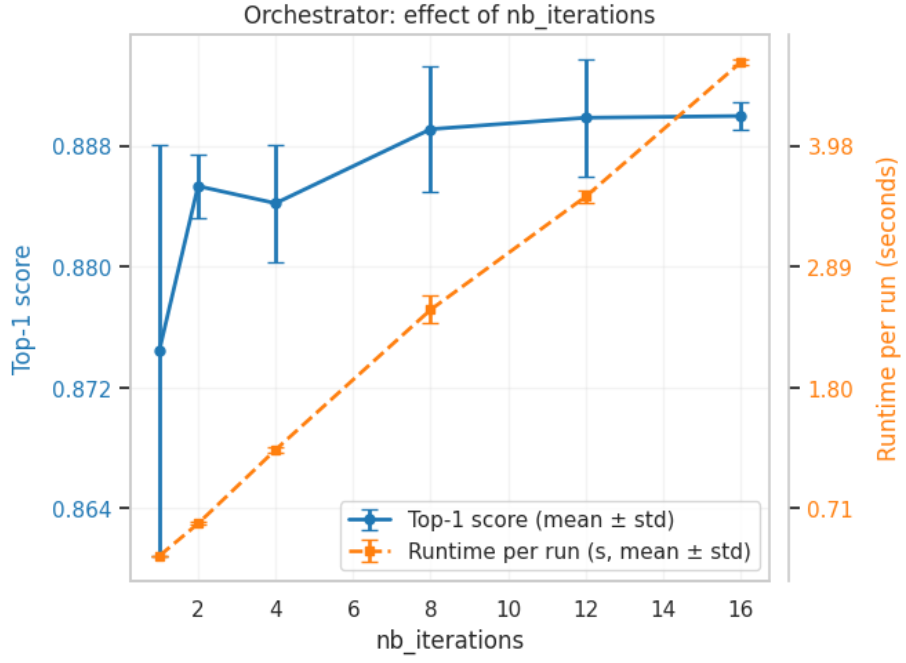
\includegraphics[width=\linewidth]{images/pipeline_effect_of_nb_iterations.png}

        \column{0.5\textwidth}
        \centering
        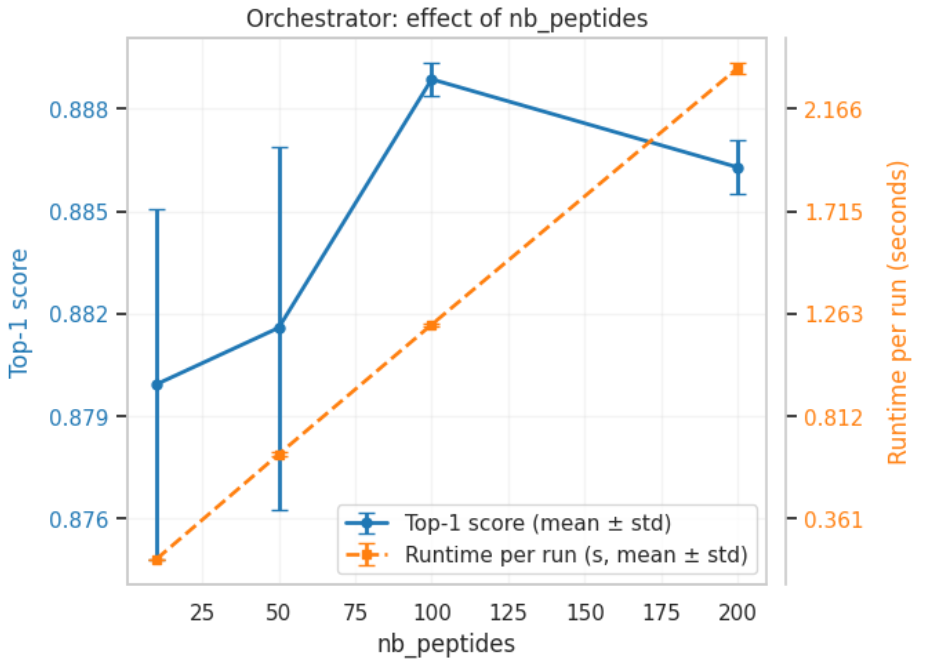
\includegraphics[width=\linewidth]{images/pipeline_effect_of_nb_peptide.png}
    \end{columns}
    \raggedleft \tiny \textcolor{gray}{Runtime: RTX 4070 (Portable), Ryzen 7350XT, 16Go RAM}

    \begin{block}{Analyse}
        \scriptsize
        Augmenter le budget de recherche améliore très légèrement la qualité mais rapidement le runtime, suggérant une possibilitée d'amélioration d'orchestrateur.
    \end{block}
\end{frame}

\begin{frame}
    \frametitle{Résultats: impact de la longueur cible}
    \begin{columns}[T,totalwidth=\textwidth]
        \column{0.60\textwidth}
        \centering
        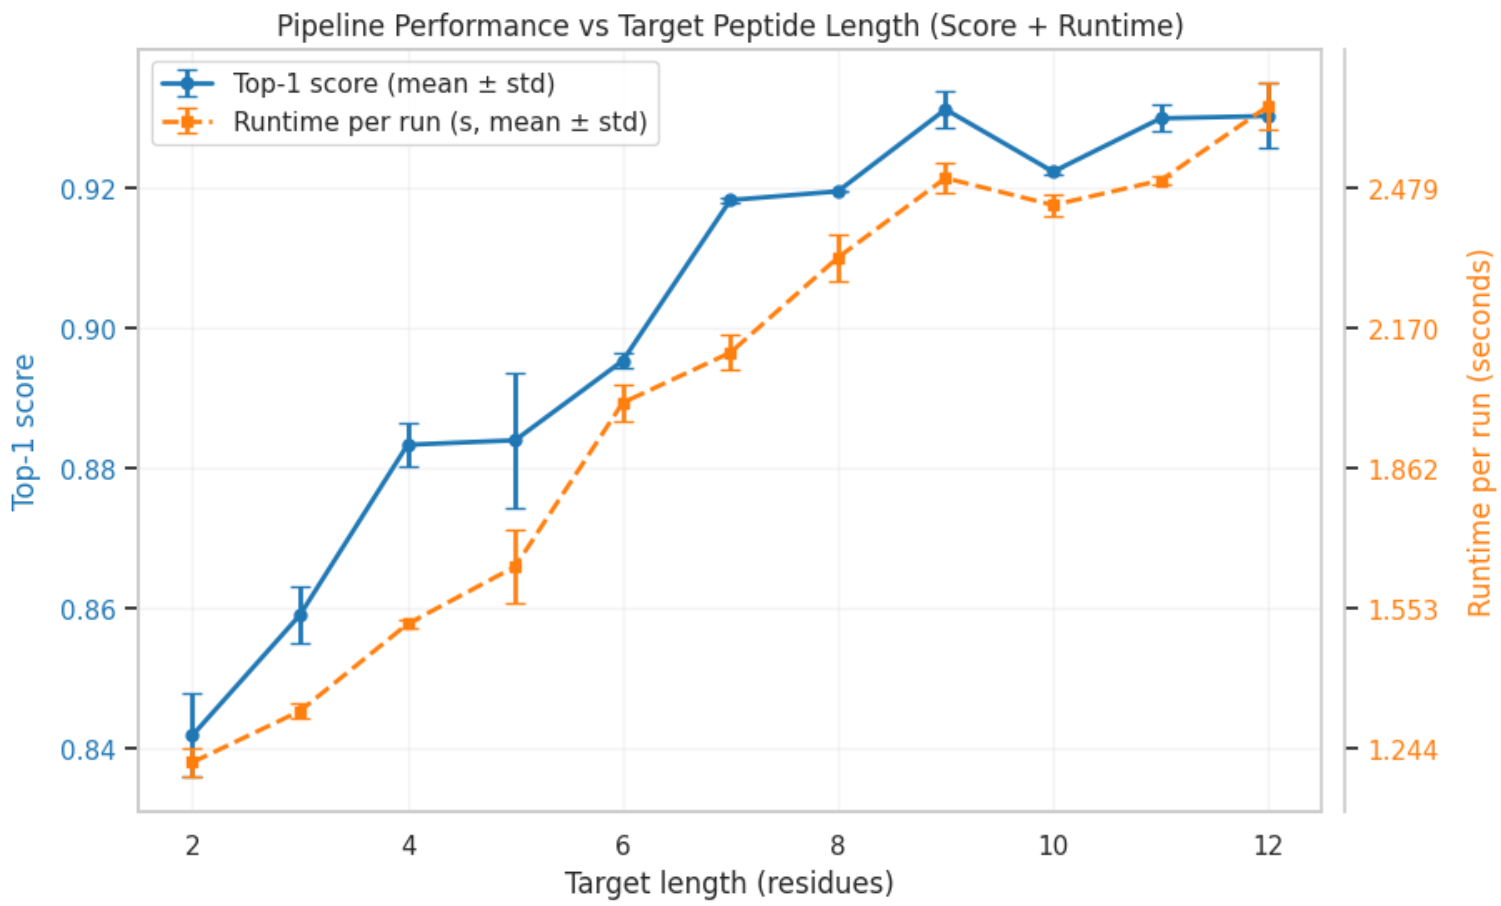
\includegraphics[width=\linewidth]{images/pipeline_performance_per_target_length.png}

        \column{0.36\textwidth}
        \begin{block}{Analyse}
            \footnotesize
            \begin{itemize}
                \item Les cibles très courtes (2--3) restent les plus difficiles.
                \item Le score remonte ensuite jusqu'à un plateau vers la longueur 11.
            \end{itemize}
        \end{block}
        
        \raggedleft \tiny \textcolor{gray}{Runtime: RTX 4070 (Portable), Ryzen 7350XT, 16Go RAM}
    \end{columns}
    \begin{alertblock}{Attention}
        \footnotesize
        Les scores élevés sur des longueurs pathologiques très courtes peuvent refléter
        une faiblesse de l'expert biologique plus qu'une plausibilité biologique réelle.
    \end{alertblock}


\end{frame}

\begin{frame}
    \frametitle{Pipeline vs baseline selon la difficulté}
    \begin{columns}[T,totalwidth=\textwidth]
        \column{0.58\textwidth}
        \centering
        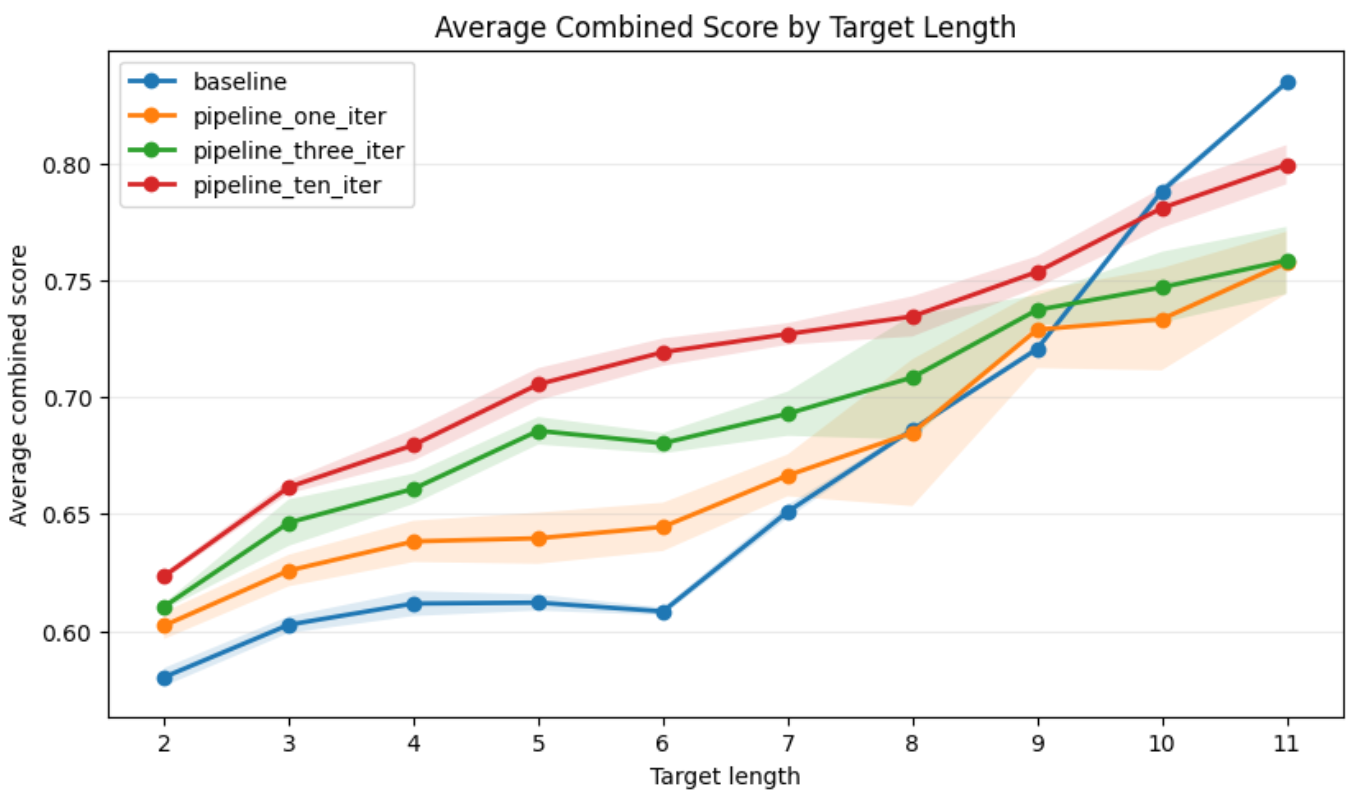
\includegraphics[width=\linewidth]{images/average_combined_score_by_target_length.png}

        \column{0.40\textwidth}
        \begin{block}{Analyse}
            \footnotesize
            \begin{itemize}
                \item Sur cibles courtes (difficiles), l'itération aide clairement
                \item Sur cibles longues (faciles), le gain n'est pas systématique
                \item Plus stable avec plus d'itérations
            \end{itemize}
        \end{block}

    \end{columns}
\end{frame}

\section{Discussion et perspectives}

\begin{frame}
    \frametitle{Discussion}
    \begin{block}{Portée des résultats}
        \footnotesize
        Le pipeline est un \textbf{PoC in silico}: les signaux chimie/biologie guident l'optimisation, mais ne remplacent pas une validation expérimentale. Les résultats sont des preuves d'ingénierie et des pistes d'amélioration, pas des conclusions biologiques définitives.
    \end{block}

    \begin{block}{Limites techniques principales}
        \footnotesize
        \begin{itemize}
            \item Contrôle conditionnel dépendant de la \textbf{qualité des labels} et des variables de conditioning fournis lors de l'entraînement.
            \item Signal biologique (ESM): bon proxy d'ordre mais \textbf{pas une vérité expérimentale}, risque d'incertitude.
            \item Orchestrateur: gains marginaux en qualité pour budgets élevés, signe d'une efficacité d'échantillonnage perfectible.
        \end{itemize}
    \end{block}
\end{frame}

\begin{frame}
    \frametitle{Perspectives}
    \begin{itemize}
        \item \textbf{Biologiste peptide-spécifique}: entraînement/fine-tuning sur jeux de données peptide-annotés pour produire un score plus discriminatif (activité et risques séparés).
        \item \textbf{Orchestrateur exploration-aware}: politiques adaptatives (exploration dynamique, sélection par incertitude/diversité) pour améliorer rendement qualité/compute.
        \item \textbf{Interface plus expressive}: LLM comme couche d'interface pour traduire objectifs utilisateurs (langage naturel) en contraintes structurées.
        \item \textbf{Chimie enrichie}: ajouter des descripteurs dérivés (SMILES, fingerprints) et intégrer évaluations de synthétisabilité.
    \end{itemize}
    \vspace{0.5em}
    \begin{center}
        \footnotesize $\implies$ Ces axes ciblent la robustesse du signal, la contrôlabilité du générateur et l'efficacité de l'orchestration.
    \end{center}
\end{frame}

\end{document}